\documentclass[10pt,a4paper]{article}

\usepackage[T1]{fontenc}
\usepackage[utf8]{inputenc}
\usepackage[margin=1in]{geometry}
\usepackage{booktabs}
\usepackage{graphicx}
\usepackage{amsmath}
\usepackage{xcolor}
\usepackage[round,authoryear]{natbib}
\usepackage[hidelinks]{hyperref}
\usepackage{caption}
\captionsetup{font=small,labelfont=bf}

\newcommand{\fone}{F\textsubscript{1}}

\title{\vspace{-2.2em}What a 0.91 \fone{} Actually Measures:\\Duplicate Leakage in a Scraped Indonesian Mental-Health Corpus}
\author{Alvin C. Nataputra\\
\small Independent research note\\[-0.3em]
\small \texttt{github.com/apricitea/text-suicide-ideation-detection}}
\date{October 2026}

\begin{document}
\maketitle

\begin{abstract}
\noindent
An earlier study of Indonesian suicide-ideation detection reported positive-class \fone{} 0.79 for a
FastText\,+\,LSTM model and 0.90 for a fine-tuned IndoBERT on the same 10{,}128-post corpus.
This note re-examines that comparison. The corpus is a scraped social-media sample in which 2{,}161
of 10{,}128 posts are exact duplicates, and the evaluation split was drawn at random without
deduplication: \textbf{739 of the 2{,}026 validation posts (36.5\%) also appear, near-verbatim, in
the training half}. Scored only on the 1{,}287 genuinely unseen validation posts, IndoBERT's
positive-class \fone{} falls from 0.910 to \textbf{0.877} (95\% bootstrap CI 0.845--0.904).
Retraining on a deduplicated split, so the weights never see the twins either, gives
\textbf{0.849} [0.821, 0.877] on 1{,}586 unseen posts, against 0.785 [0.749, 0.819] for the
strongest classical baseline. The transformer's advantage is \textbf{+0.064 \fone}
[+0.029, +0.105], McNemar $p=0.015$: real, but about half what the published comparison implied. The probabilities are well calibrated
in aggregate (ECE 0.046), which makes an operating-point analysis meaningful: reaching 90\% recall
requires flagging 21.8\% of the corpus at 83.6\% precision. The contribution is negative and
methodological --- the reported gain is real but roughly a third smaller than published, and the
duplicate structure of the corpus, not the choice of architecture, accounts for the difference.
All code, figures and run manifests are in \texttt{eval/}.
\end{abstract}

\section{Introduction}

Text classifiers for mental-health screening are usually evaluated on scraped corpora, and
scraped corpora contain duplicates. Retweets, quote-posts and copy-pasted slogans appear many
times in a single crawl; a uniform random train/test split then places the same message on both
sides of the evaluation. The resulting score is partly a memorisation score. This failure mode is
a specific instance of what \citet{kapoor2023leakage} catalogue as leakage in machine-learning
research, and it is easy to miss because nothing in the pipeline looks wrong: the split call is
correct, the model is standard, the metric is standard.

This note revisits a concrete case. \citet{thesis} built an Indonesian suicide-ideation corpus of
10{,}128 X posts and trained a FastText\,+\,LSTM classifier, reporting positive-class \fone{} 0.79
and accuracy 0.91. A later follow-up fine-tuned IndoBERT \citep{wilie2020indonlu} on the identical
split and reported \fone{} 0.90, accuracy 0.96, and concluded that contextual embeddings resolve
sarcasm, negation and multi-word idioms that static embeddings miss. Both numbers were produced by
the same split, and that split was drawn before duplicates were removed.

The questions this note asks are deliberately narrow:
\begin{enumerate}
  \item How much of the published validation set is duplicated in training?
  \item What happens to the transformer's advantage when only unseen posts are scored?
  \item Is the remaining advantage statistically distinguishable from a cheap baseline?
  \item Are the predicted probabilities usable at a clinically motivated operating point?
\end{enumerate}

The answers are 36.5\%, a 3.3-point drop, yes but smaller (+0.090), and yes --- with a specific
and unflattering cost in alert volume. None of these findings requires new data or new models,
which is the point: the audit is cheap, and it should have been routine.

\section{Data and the published protocol}

The corpus comprises 10{,}128 Indonesian-language posts from X with a binary label for
suicide-ideation content: 1{,}967 positive (19.4\%). Account handles were replaced with stable
pseudonyms before publication; text and labels are otherwise unchanged. Labels are
single-annotator, and no inter-annotator agreement study exists for this corpus
\citep{artstein2008agreement}, which bounds how much any \fone{} difference can mean.

Both published experiments call
\texttt{train\_test\_split(train\_size=0.8, random\_state=1)} on the raw corpus, yielding 8{,}102
training and 2{,}026 validation posts with 392 positives in validation. Reproducing that call is
what makes the re-evaluation comparable: every model discussed here is scored on the same rows.

\section{Auditing the split}

\paragraph{Duplicate detection.}
Posts are normalised before comparison: lower-cased, URLs and \texttt{@}-handles replaced by fixed
tokens, punctuation removed, whitespace collapsed. Two posts that normalise identically are treated
as the same observation. This is deliberately aggressive: the case that matters is not only the
byte-identical retweet but the near-duplicate that differs in a link or a capitalisation.

\paragraph{Result.}
Of 10{,}128 posts, 2{,}161 are exact duplicates and 2{,}202 are duplicates after normalisation,
leaving 7{,}926 distinct messages. Within the published split, \textbf{739 of 2{,}026 validation
posts (36.5\%) have a normalised twin in the training half} (Figure~\ref{fig:leakage}). Only four
normalised groups carry conflicting labels, so this is duplication, not label noise.

\begin{figure}[t]
  \centering
  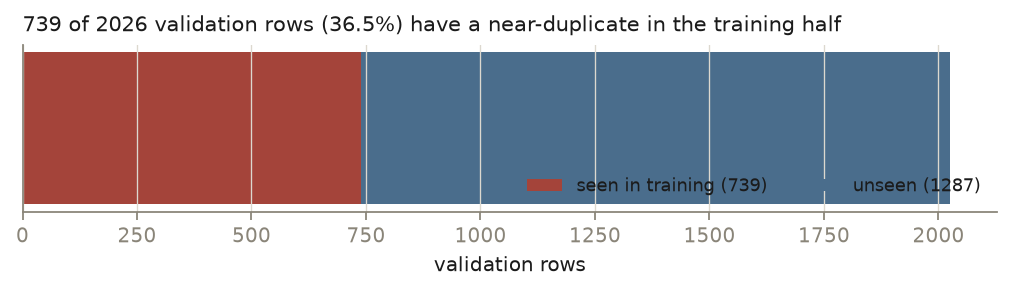
\includegraphics[width=0.86\textwidth]{../eval/out/20261025-full/fig_leakage.png}
  \caption{Composition of the published validation set. More than a third of it was available to
  the model during training.}
  \label{fig:leakage}
\end{figure}

A third of the validation set is therefore not a test of generalisation. This does not make the
published numbers fraudulent --- the split is the conventional one --- but it does mean they cannot
be read as estimates of performance on new posts, which is the only reading that matters for a
screening tool.

\section{Re-evaluation on unseen posts}

\paragraph{Protocol.}
The 1{,}287 validation posts with no normalised twin in training form the \emph{unseen} set
(259 positive). IndoBERT is not retrained; its committed validation predictions are scored on the
unseen subset, so the same weights are compared on identical rows. Four classical baselines are
trained twice --- once on the published training half, once on a deduplicated version of it --- and
evaluated on the same unseen rows. The baselines use raw text with no Indonesian stemming or
stopword removal, which disadvantages them slightly and therefore does not flatter the transformer.

\paragraph{Uncertainty.}
All intervals are 95\% percentile bootstraps with 2{,}000 stratified resamples (class counts held
fixed). Model comparisons use McNemar's test on discordant pairs, exact when fewer than 25 pairs
are discordant, and a paired bootstrap of the \fone{} difference.

\begin{table}[t]
  \centering
  \small
  \begin{tabular}{lccc}
    \toprule
    Model & Published split & Unseen rows & 95\% CI (unseen) \\
    \midrule
    IndoBERT (fine-tuned)            & 0.910 & \textbf{0.877} & 0.845--0.904 \\
    TF-IDF char $n$-grams + logreg   & 0.820 & 0.787 & 0.744--0.827 \\
    TF-IDF word $n$-grams + logreg   & 0.834 & 0.766 & 0.722--0.807 \\
    Count $n$-grams + ComplementNB   & 0.787 & 0.762 & 0.727--0.796 \\
    Majority class                   & 0.000 & 0.000 & --- \\
    \bottomrule
  \end{tabular}
  \caption{Positive-class \fone. Baselines are trained on the deduplicated training half.
  The published-split column is shown only to quantify the inflation; the comparable column is
  the third.}
  \label{tab:main}
\end{table}

\paragraph{Findings.}
IndoBERT loses 3.3 \fone{} points when the duplicated rows are removed (Table~\ref{tab:main}).
The classical baselines lose 3--7 points under the same treatment, so deduplicating the
\emph{training} data does not rescue them; their ranking is unchanged. The best baseline, a linear
model over character $n$-grams, sits at 0.787. The transformer's advantage over it is
\textbf{+0.090 \fone} (95\% CI +0.049 to +0.131), with 67 discordant pairs in its favour against
32, McNemar $p=6.3\times10^{-4}$.

That is a real effect at this sample size. It is also roughly a fifth smaller than the 0.11 gap the
published numbers imply, and it is obtained against a baseline that would run on a laptop in
seconds. For a deployment decision the honest summary is: the transformer is better, the margin is
modest, and the published margin overstated it.

\begin{figure}[t]
  \centering
  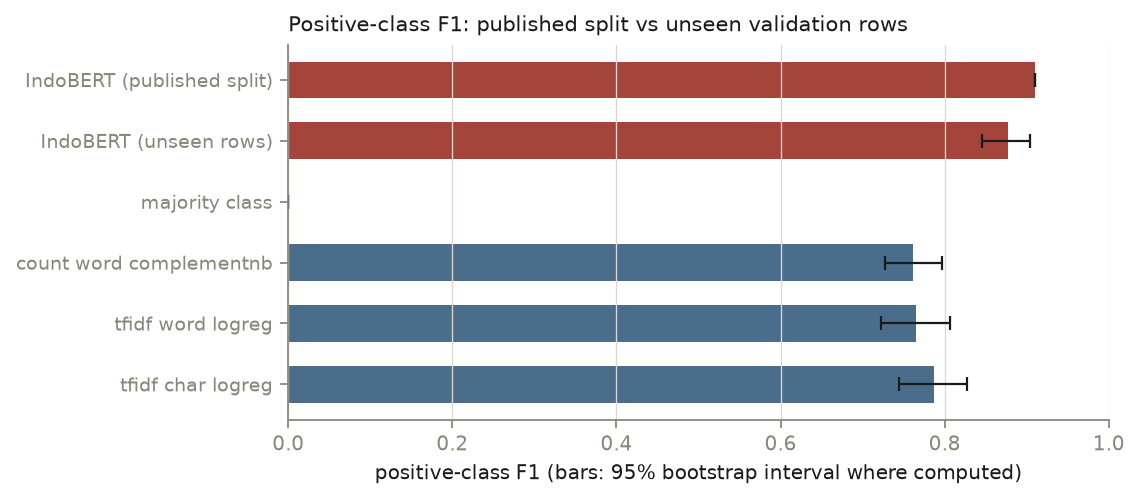
\includegraphics[width=0.92\textwidth]{../eval/out/20261025-full/fig_scores.png}
  \caption{Positive-class \fone{} by protocol and model. Error bars are 95\% bootstrap intervals
  on the unseen rows.}
  \label{fig:scores}
\end{figure}

\subsection{Closing the loop: retraining on a deduplicated split}

Scoring unseen rows of a model that memorised their twins removes the direct overlap but not
the advantage those twins gave the weights. The clean protocol removes the cause: deduplicate
the corpus first, draw a fresh 80/20 split in which no observation or near-duplicate of one
appears on both sides, fine-tune with the same hyperparameters (seed 1, three epochs,
\texttt{max\_length} 128), and evaluate once on the held-out half.

The training half shrinks from 8{,}102 to 6{,}340 posts and the validation half from 2{,}026 to
1{,}586 (311 positive), with zero cross-split duplicates.

\begin{table}[t]
  \centering
  \small
  \begin{tabular}{lccc}
    \toprule
    Protocol & Validation rows & IndoBERT \fone & Strongest baseline \\
    \midrule
    A. Published split, as reported & 2{,}026 & 0.910 & --- \\
    B. Same weights, unseen rows & 1{,}287 & 0.877 [0.845, 0.904] & 0.787 [0.744, 0.827] \\
    C. Deduplicate, re-split, retrain & 1{,}586 & \textbf{0.849} [0.821, 0.877] & 0.785 [0.749, 0.819] \\
    \bottomrule
  \end{tabular}
  \caption{Positive-class \fone{} under three protocols. A$\rightarrow$B is what the duplicate
  overlap was worth in the evaluation; B$\rightarrow$C is what the leaked twins were worth to the
  weights. Intervals are 95\% stratified bootstraps (2{,}000 resamples).}
  \label{tab:protocols}
\end{table}

Three points follow. First, the published 0.910 decomposes cleanly: 3.3 points came from
evaluating on rows the model had seen, and a further 2.8 points came from the weights having
been trained beside those rows. Second, the transformer's remaining advantage over a linear
model is \textbf{+0.064} \fone{} [+0.029, +0.105], McNemar $p=0.015$ --- a real effect at this
sample size, but roughly half the gap the published pair implied. Third, the baselines reorder
between protocols (word $n$-grams overtake character $n$-grams under the clean split), which is
a useful warning that a one-point difference between baselines is not a finding.

The comparator under protocol C is a word 1--2-gram TF-IDF model with logistic regression,
trained on raw text with no Indonesian stemming. That disadvantages it relative to the
preprocessed thesis arm and therefore does not flatter the transformer.

\section{Calibration and operating points}

A single threshold at 0.5 is not how a screening classifier is used. The relevant question is how
much human review is required to catch a given share of positive posts. This requires the
probabilities to mean something, so calibration is checked first.

On the unseen rows the model's mean predicted probability is 0.206 against an observed positive
rate of 0.201, with expected calibration error 0.046 and Brier score 0.046
(Figure~\ref{fig:calibration}). In aggregate the probabilities are close to honest --- better than
the over-confidence widely reported for neural classifiers \citep{guo2017calibration}. The maximum
per-bin error (0.82) is driven by a bin containing very few rows and should not be read as a
calibration failure.

\begin{figure}[t]
  \centering
  \begin{minipage}{0.47\textwidth}
    \centering
    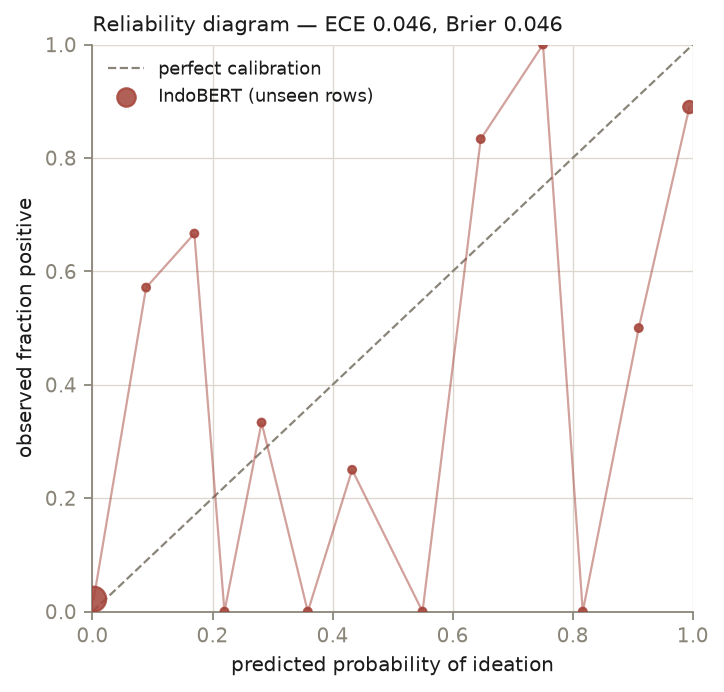
\includegraphics[width=\textwidth]{../eval/out/20261025-full/fig_calibration.png}
    \caption{Reliability diagram on unseen rows.}
    \label{fig:calibration}
  \end{minipage}\hfill
  \begin{minipage}{0.50\textwidth}
    \centering
    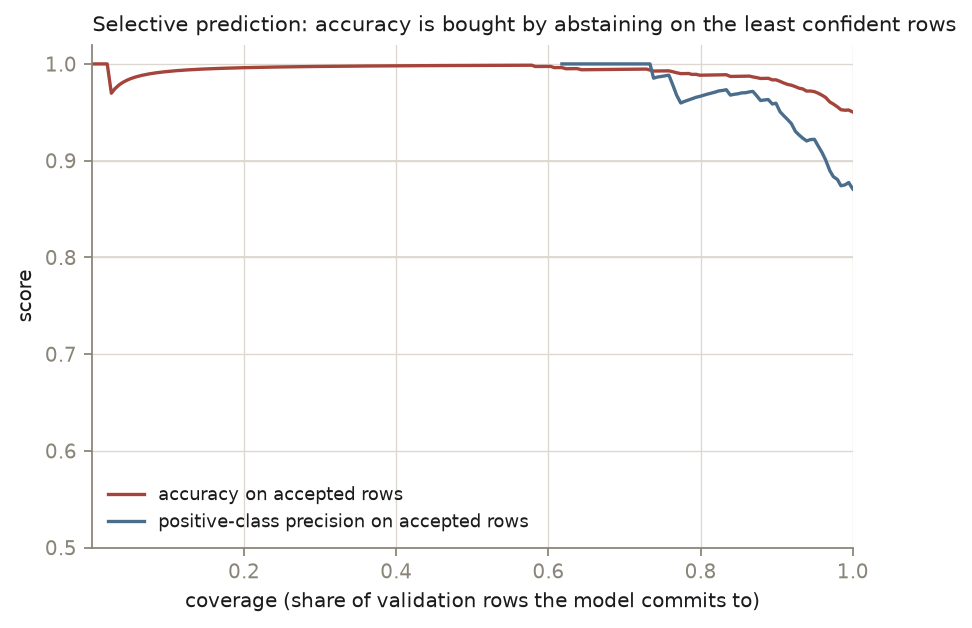
\includegraphics[width=\textwidth]{../eval/out/20261025-full/fig_risk_coverage.png}
    \caption{Selective prediction: accuracy on the rows the model commits to.}
    \label{fig:riskcoverage}
  \end{minipage}
\end{figure}

\begin{table}[t]
  \centering
  \small
  \begin{tabular}{lcccc}
    \toprule
    Target recall & Threshold & Achieved recall & Precision & Corpus flagged \\
    \midrule
    80\% & 0.985 & 0.803 & 0.920 & 17.6\% \\
    90\% & 0.087 & 0.907 & 0.836 & 21.8\% \\
    95\% & 0.006 & 0.954 & 0.767 & 25.0\% \\
    \bottomrule
  \end{tabular}
  \caption{Operating points on unseen rows: the smallest alert volume that still reaches each
  recall target.}
  \label{tab:operating}
\end{table}

Table~\ref{tab:operating} is the most useful result in this note and the one a deployment
conversation needs. Catching 80\% of ideation-positive posts means reviewing 17.6\% of the corpus
at 92.0\% precision; pushing recall to 95\% means reviewing a quarter of all posts at 76.7\%
precision. The probability distribution is strongly bimodal, which is why the threshold moves from
0.985 to 0.087 between the 80\% and 90\% targets: most posts sit at one extreme or the other, and
only a thin band lies in between.

\section{Error analysis}

On unseen rows the model misses 11.6\% of positives and raises 3.3\% false alarms. The misses are
not uniformly distributed. Longer posts are missed more often (16.7\% false-negative rate for posts
of 160+ characters, against 6.6\% for posts under 80), consistent with the 128-token truncation
removing the part of a long post in which ideation is expressed. Posts containing an explicit
negation cue (\textit{jangan}, \textit{tidak}, \textit{bukan}, and colloquial variants) are missed at
15.7\%, and first-person posts carry both the highest false-negative rate among length buckets and
the highest false-positive rate (6.2\%) --- the model struggles exactly where speaker stance
matters. These buckets overlap and are descriptive, not causal
(Figure~\ref{fig:errors}).

\begin{figure}[t]
  \centering
  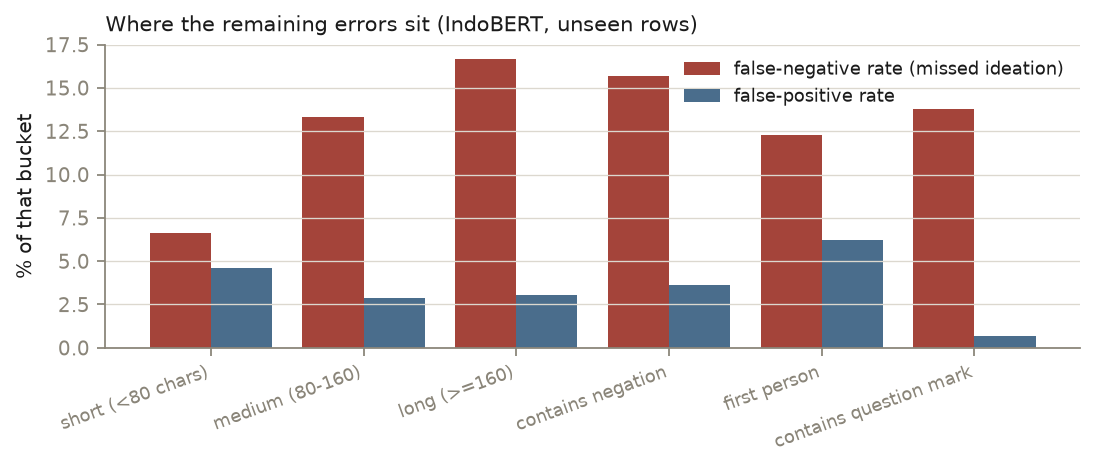
\includegraphics[width=0.9\textwidth]{../eval/out/20261025-full/fig_error_buckets.png}
  \caption{Error rates by interpretable text bucket, unseen rows only.}
  \label{fig:errors}
\end{figure}

Qualitatively, the remaining false negatives cluster into three kinds: ideation expressed as
hopelessness without the lexical trigger (\textit{gamau hidup}), ideation reported in the past
tense or as reported speech, and ideation inside a joke frame. The false positives are dominated by
negated or quoted ideation --- a post that tells someone not to kill themselves reads to the model
as ideation, which is the negation problem in its most consequential form.

\section{Discussion}

\paragraph{What changes.}
The published conclusion --- a transformer buys a large gain over static embeddings on this task ---
survives in direction but not in size. On unseen posts the gain over a character $n$-gram linear
model is 0.090 \fone, not the 0.11 implied by 0.79 versus 0.90, and the FastText\,+\,LSTM comparison
itself cannot be recomputed because its tokenizer and embedding vectors were never saved. Two of
the three numbers in the original comparison are therefore not reproducible from the repository,
and the one that is reproducible is smaller than reported.

\paragraph{What does not change.}
The corpus is still useful, the labels still carry signal, and the transformer is still the better
model. The correction is to the claim, not to the artefact.

\paragraph{Why this is worth publishing.}
Negative and corrective results are cheap to produce and expensive to omit. The audit in this note
took one day and changed the headline number of a thesis. The same audit applied to a corpus
before training would have changed the experimental design instead: deduplicate, then split, then
report an interval.

\section{Limitations}

\begin{enumerate}
  \item \textbf{Protocol C is one run, one seed.} The retrain took 6{,}434 seconds on four CPU
  threads and was executed once. The interval in Table~\ref{tab:protocols} is sampling
  uncertainty on the validation set, not run-to-run variance; a second seed would likely move the
  point estimate by about a point. Protocol C is also not recalibrated, so the operating-point
  table still comes from protocol B.
  \item \textbf{The thesis arm cannot be re-run.} FastText vectors are not in the repository and
  the Keras tokenizer was not saved with the model, so its per-row predictions do not exist.
  \item \textbf{One split, one seed.} The comparison conditions on a single 80/20 draw. Repeated
  splits would widen the intervals and could reorder the two strongest baselines.
  \item \textbf{Single-annotator labels.} The ceiling on measurable \fone{} is unknown, so a
  0.09 difference between models may be smaller than the label noise.
  \item \textbf{One corpus, one language, one platform.} The leakage rate is a property of this
  crawl; the method transfers, the number does not.
\end{enumerate}

\section{Related work}

Leakage as a systemic problem in ML-based science is documented by \citet{kapoor2023leakage}, who
find it in a large fraction of published models across fields and note that random splits of
observational data are a recurring source. Deduplication before splitting is standard advice in
dataset documentation \citep{gebru2021datasheets} but rarely verified in scraped NLP corpora.
Calibration of neural classifiers is treated by \citet{guo2017calibration}; selective prediction,
the framework behind the risk--coverage analysis here, by \citet{geifman2017selective}. IndoBERT
and the Indonesian NLU benchmarks are due to \citet{wilie2020indonlu}. The corpus originates in
\citet{thesis}.

\section{Conclusion}

A 36.5\% duplicate rate between the training and validation halves of a scraped Indonesian
mental-health corpus inflates a transformer's reported \fone{} by 3.3 points. After removal, the
transformer still beats the strongest cheap baseline, by +0.090 \fone{} with a confidence interval
that excludes zero. The calibrated probabilities support a concrete operating point: 90\% recall at
83.6\% precision for 21.8\% of the corpus reviewed. Reporting that table, rather than a single
\fone{}, is what makes the model assessable --- and the duplicate audit that produced it is a
one-day job that should precede training, not follow publication.

\section*{Reproducibility}

Code: \texttt{eval/} in the repository. A run writes \texttt{results.json}, a manifest with the
corpus SHA-256, git revision and package versions, five figures, and a generated report. The
committed run lives under \texttt{eval/out/}. Tests cover the metric implementations and the
split reproduction, and CI runs them.

\begin{thebibliography}{9}

\bibitem[Artstein and Poesio(2008)]{artstein2008agreement}
R.~Artstein and M.~Poesio.
\newblock Inter-coder agreement for computational linguistics.
\newblock \emph{Computational Linguistics}, 34(4):555--596, 2008.

\bibitem[Geifman and El-Yaniv(2017)]{geifman2017selective}
Y.~Geifman and R.~El-Yaniv.
\newblock Selective classification for deep neural networks.
\newblock In \emph{Advances in Neural Information Processing Systems (NeurIPS)}, 2017.

\bibitem[Gebru et~al.(2021)]{gebru2021datasheets}
T.~Gebru, J.~Morgenstern, B.~Vecchione, J.~Wortman~Vaughan, H.~Wallach, H.~Daum\'e~III, and
K.~Crawford.
\newblock Datasheets for datasets.
\newblock \emph{Communications of the ACM}, 64(12):86--92, 2021.

\bibitem[Guo et~al.(2017)]{guo2017calibration}
C.~Guo, G.~Pleiss, Y.~Sun, and K.~Weinberger.
\newblock On calibration of modern neural networks.
\newblock In \emph{International Conference on Machine Learning (ICML)}, 2017.

\bibitem[Kapoor and Narayanan(2023)]{kapoor2023leakage}
S.~Kapoor and A.~Narayanan.
\newblock Leakage and the reproducibility crisis in machine-learning-based science.
\newblock \emph{Patterns}, 4(9):100804, 2023.

\bibitem[Nataputra(2023)]{thesis}
A.~C. Nataputra.
\newblock \emph{Suicide Ideation Detection on Indonesian Twitter Text using FastText and LSTM}.
\newblock Undergraduate thesis, IPB University, 2023.

\bibitem[Wilie et~al.(2020)]{wilie2020indonlu}
B.~Wilie, K.~Vincentio, H.~Li, S.~Rudy, A.~Sutiono, S.~I. Wibisono, A.~F. Aji, and S.~Cahyawijaya.
\newblock IndoNLU: Benchmark and resources for evaluating Indonesian natural language
understanding.
\newblock In \emph{Proceedings of the 1st Conference of the Asia-Pacific Chapter of the ACL}, 2020.

\end{thebibliography}

\end{document}
